\documentclass[11pt]{article}
\usepackage{fullpage}
\usepackage{amsfonts}
\usepackage{amssymb}
\usepackage{mdwlist}
\usepackage[usenames,dvipsnames]{xcolor}
\usepackage{tikz}
\usepackage{enumerate}



%Formatting


\setlength{\topmargin}{0in}
\setlength{\oddsidemargin}{0 in}
\setlength{\evensidemargin}{0 in}
\setlength{\textwidth}{6.5 in}
\setlength{\textheight}{8.5 in}
\setlength{\headsep}{0.75 in}
\setlength{\parindent}{0 in}
\setlength{\parskip}{0.05 in}

%Theorems, proofs, etc.

\newtheorem{theorem}{Theorem}
\newtheorem{lemma}[theorem]{Lemma}
\newtheorem{corollary}[theorem]{Corollary}
\newtheorem{proposition}[theorem]{Proposition}
\newtheorem{claim}[theorem]{Claim}
\newtheorem{exercise}{Exercise}
\newtheorem{conjecture}{Conjecture}
\newtheorem{example}{Example}
\newtheorem{remark}{Remark}
\newtheorem{definition}[theorem]{Definition}
\newenvironment{proof}{\noindent {\sc Proof:}}{$\Box$\medskip} 
\newtheorem{question}{Open Question}
\newtheorem{problem}{Problem}



%% Macros for complexity theory notation
%% Complexity classes
\newcommand\p{\mbox{\bf P}}
\newcommand\np{\mbox{\bf NP}}
\newcommand\am{\mbox{\bf AM}}
\newcommand\ma{\mbox{\bf MA}}
\newcommand\distnp{\mbox{\bf DistNP}}
\newcommand\cnp{\mbox{\bf coNP}}
\newcommand\corp{\mbox{\bf coRP}}
\newcommand\sigmatwo{\mbox{\bf $\Sigma_2$}}
\newcommand\sigmathree{\mbox{\bf $\Sigma_3$}}
\newcommand\pitwo{\mbox{\bf $\Pi_2$}}
\newcommand\rp{\mbox{\bf RP}}
\newcommand\zpp{\mbox{\bf ZPP}}
\newcommand\bpp{\mbox{\bf BPP}}
\newcommand\ph{\mbox{\bf PH}}
\newcommand\pspace{\mbox{\bf PSPACE}}
\newcommand\npspace{\mbox{\bf NPSPACE}}
\newcommand\aczero{\mbox{\bf AC$^0$}}
\newcommand\dl{\mbox{\bf L}}
\newcommand\nl{\mbox{\bf NL}}
\newcommand\rl{\mbox{\bf RL}}
\newcommand\sll{\mbox{\bf SL}}
\newcommand\bpl{\mbox{\bf BPL}}
\newcommand\conl{\mbox{\bf coNL}}
\newcommand\sharpp{\mbox{\#{\bf P}}}
\newcommand\parityp{\mbox{$\oplus$ {\bf P}}}
\newcommand\ip{\mbox{\bf IP}}
\newcommand\pcp{\mbox{\bf PCP}}
\newcommand\dtime{\mbox{\bf DTIME}}
\newcommand\ntime{\mbox{\bf NTIME}}
\newcommand\bptime{\mbox{\bf BPTIME}}
\newcommand\dspace{\mbox{\bf SPACE}}
\newcommand\nspace{\mbox{\bf NSPACE}}
\newcommand\cnspace{\mbox{\bf coNSPACE}}
\newcommand\exptime{\mbox{\bf EXPTIME}}
\def\exp{\mbox{\bf EXP}}
\def\ep{\mbox{\bf E}}
\newcommand\nexptime{\mbox{\bf NEXPTIME}}
\newcommand\genclass{\mbox{$\cal C$}}
\newcommand\cogenclass{\mbox{\bf co$\cal C$}}
\newcommand\size{\mbox{\bf SIZE}}

\def\phi{\varphi}

%%Computational problems

\newcommand\sat{\mbox{SAT}}
\newcommand\tsat{\mbox{3SAT}}
\newcommand\tqbf{\mbox{TQBF}}
\newcommand\permp{\mbox{\sc Permanent}}
\def\perm{\operatorname{perm}}

%% Notation for integers, natural numbers, reals, fractions, sets, cardinalities
%%and so on

\newcommand\Z{\mbox{$\mathbb Z$}}
\newcommand\N{\mbox{$\mathbb N$}}
\newcommand\R{\mbox{$\mathbb R$}}
\newcommand\F{\mbox{$\mathcal{F}$}}
\newcommand\B{\{0,1\}}      % boolean alphabet  use in math mode
\newcommand\Bs{\{0,1\}^*}   % B star            use in math mode
\def\H{\{-1,1\}}      
\def\S{{\cal S}}

\newcommand{\bzero}{{\bf 0}}


\newcommand\true{\mbox{\sc True}}
\newcommand\false{\mbox{\sc False}}

\newcommand{\marginlabel}[1]%
{\mbox{}\marginpar{\it{\raggedleft\hspace{0pt}#1}}}
\newcommand\poly{\mbox{poly}}  %usage \poly(n)
\newcommand{\floor}[1]{\lfloor\, $#1$\,\rfloor}
\newcommand{\ceil}[1]{\lceil\, $#1$\,\rceil}
\newcommand{\comp}[1]{\overline{#1}}


%\newcommand\to{\rightarrow} 
\newcommand\xor{\oplus}
\newcommand\bigxor{\bigoplus}
\newcommand{\logred}{\leq_{\log}}
\def\implies{\Rightarrow}


%% probability stuff

\newcommand\E{\mathop\mathbb{E}}
\newcommand\pr{\mathop{\bf {Pr}}}
\newcommand\var{\mathop{\bf Var}}


%% macros to write pseudo-code

\newlength{\pgmtab}  %  \pgmtab is the width of each tab in the
\setlength{\pgmtab}{1em}  %  program environment
 \newenvironment{program}{\renewcommand{\baselinestretch}{1}%
\begin{tabbing}\hspace{0em}\=\hspace{0em}\=%
\hspace{\pgmtab}\=\hspace{\pgmtab}\=\hspace{\pgmtab}\=\hspace{\pgmtab}\=%
\hspace{\pgmtab}\=\hspace{\pgmtab}\=\hspace{\pgmtab}\=\hspace{\pgmtab}\=%
\+\+\kill}{\end{tabbing}\renewcommand{\baselinestretch}{\intl}}
\newcommand {\BEGIN}{{\bf begin\ }}
\newcommand {\ELSE}{{\bf else\ }}
\newcommand {\IF}{{\bf if\ }}
\newcommand {\FOR}{{\bf for\ }}
\newcommand {\TO}{{\bf to\ }}
\newcommand {\DO}{{\bf do\ }}
\newcommand {\WHILE}{{\bf while\ }}
\newcommand {\ACCEPT}{{\bf accept}}
\newcommand {\REJECT}{\mbox{\bf reject}}
\newcommand {\THEN}{\mbox{\bf then\ }}
\newcommand {\END}{{\bf end}}
\newcommand {\RETURN}{\mbox{\bf return\ }}
\newcommand {\HALT}{\mbox{\bf halt}}
\newcommand {\REPEAT}{\mbox{\bf repeat\ }}
\newcommand {\UNTIL}{\mbox{\bf until\ }}
\newcommand {\TRUE}{\mbox{\bf true\ }}
\newcommand {\FALSE}{\mbox{\bf false\ }}
\newcommand {\FORALL}{\mbox{\bf for all\ }}
\newcommand {\DOWNTO}{\mbox{\bf down to\ }}


%%%%%%%%    FALL'05
\newcommand{\coursenum}{CS294}
\newcommand{\coursename}{Pseudorandomness and Combinatorial Constructions}
\newcommand{\courseprof}{Professor Luca Trevisan}



%%%%%%%%%%%%%%%%%%%%%%%%%%%%%%%%%%%%%%%%%%%%%%%%%%%%%%%%%%%%%%%%%%%%%%%%%%%
%%%%%%%%%%%%%%%%%%%%%%%%%%%%%%%%%%%%%%%%%%%%%%%%%%%%%%%%%%%%%%%%%%%%%%%%%%%




\newlength{\tpush}
\setlength{\tpush}{2\headheight}
\addtolength{\tpush}{\headsep}


\newcommand{\handout}[3]{\noindent\vspace*{-\tpush}\newline\parbox{\textwidth}
{U.C. Berkeley  \hfill Handout N#1 \newline
\coursenum : \coursename \hfill #2 \newline
\courseprof \hfill #3 \newline
\mbox{}\hrulefill\mbox{}}\vspace*{1ex}\mbox{}\newline
\bigskip
\begin{center}{\Large\bf Notes for Lecture #1}\end{center}
\bigskip}


\newcommand{\problemset}[2]{\noindent\vspace*{-\tpush}\newline\parbox{\textwidth}
{U.C. Berkeley --- \coursenum : \coursename \hfill Handout #1 \newline
\courseprof \hfill #2 \newline
\mbox{}\hrulefill\mbox{}}\vspace*{1ex}\mbox{}\newline
\bigskip
\bigskip}



















\begin{document}
\ptitle{Problem Set 3}{February 5, 2015}
This problem set is due on Friday, February 13, by 5pm. Please submit your solution online using bcourses,
as a pdf file.
You can type your solution, or handwrite it. If you handwrite it, then either
scan it or take a good resolution picture of each page and then collate the pictures
and export them to a {\em single} pdf file.
\bigskip
\hrule



\section*{Problem 1: Minimal Automata (10/100)}
Consider the language $L=\{x\in\{0,1\}^*:$ the number of 1's in $x$ is a multiple of 3$\}$.  Draw a minimal DFA with states labeled with the equivalence classes [$\varepsilon$], [1], and [11] defined by indistinguishability over $L$.

\section*{Problem 2: Regular? (20/100)}

Are the following languages regular?  If so, draw a minimal DFA for it with each state labeled with its corresponding equivalence class (signified by a representative for that class under the indistinguishability relation).  If not, prove this with the Myhill-Nerode theorem by exhibiting infinitely many distinguishable strings.

\begin{enumerate}[a)]
\item $L=\{x\in\{a,b\}^*:$ the number of $b$'s in $x$ has a remainder of 3 when divided by 5$\}$

\item $L=\{x\in\{a,b\}^*:$ the number of $a$'s in $x$ is twice the number of $b$'s in $x\}$

\item $L=\{x\oplus y\ominus z:x,y,z\in\{0,1\}^*,$ bin$(x)+$bin$(y)=$bin$(z)\}$ for $\Sigma=\{0,1,\oplus,\ominus\}$.  And bin$(x)$ for $x\in\{0,1\}^*$ is the number associated with $x$ when interpreted as a binary number.

\item $L=\{x\in\{0,1\}^*: x$ ends in 101$\}$
\end{enumerate}



\section*{Problem 3: State Minimization (30/100)}

Consider the following automaton.  Find the minimal equivalent DFA.\\

\begin{tikzpicture}

\node[draw,circle,minimum size=1cm] (node0) at (0,0) {};
\node[draw,circle,minimum size=.8cm] at (0,0) {};

\node[draw,circle,minimum size=1cm] (node1) at (3,0) {};

\node[draw,circle,minimum size=1cm] (node2) at (6,0) {};

\node[draw,circle,minimum size=1cm] (redundant0) at (9,0) {};
\node[draw,circle,minimum size=.8cm] at (9,0) {};

\node[draw,circle,minimum size=1cm] (redundant1) at (4,-3) {};


\node (label) at (-2, 0) {start};
\path [-latex] (label) edge (node0);

\path [-latex] (node0) edge [bend left] node[above] {a} (node1);
\path [-latex] (node0) edge [bend right=45] node[below] {b} (node2);

\path [-latex] (node1) edge [bend left=45] node[above] {b} (redundant0);
\path [-latex] (node1) edge [bend left] node[above] {a} (node2);

\path [-latex] (node2) edge [bend left] node[above] {b} (node1);
\path [-latex] (node2) edge [bend left] node[above] {a} (redundant0);

\path [-latex] (redundant0) edge [bend left] node[below] {a} (redundant1);
\path [-latex] (redundant0) edge [bend left] node[above] {b} (node2);

\path [-latex] (redundant1) edge [bend left] node[below] {b} (node0);
\path [-latex] (redundant1) edge node[below] {a} (node2);
\end{tikzpicture}


\section*{Problem 4: Classes (40/100)}

Let $k$ be an integer, and define $L_k$ to be the language of strings
over $\{ 0,1\}$ that have a 1 in the $k$th-to-last position. Prove that $L_k$ is regular and that every DFA for $L_k$ has exponentially many states with respect to $k$.  Prove that $L_k$ has an NFA with $O(k)$ states and a Regular Expression of length $O(k)$.

\end{document}